\begin{block}{Problem Statement}
  Consider two individuals with different financial habits:
  \begin{itemize}
    \item \textbf{Person A}: Missed 2 credit card payments last year.
    \item \textbf{Person B}: Uses 85\% of available credit limit every month.
  \end{itemize}
  Which behavior falls in the generally higher-weighted FICO category? Can the category percentages alone tell us which person loses more score points?
\end{block}

\vspace{0.5em}
\centering
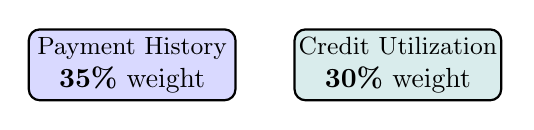
\begin{tikzpicture}[scale=0.75]
  \draw[fill=blue!15, rounded corners, thick] (0,0) rectangle (3.5,1.2) node[midway, align=center] {\small Payment History\\ \textbf{35\%} weight};
  \draw[fill=teal!15, rounded corners, thick] (4.5,0) rectangle (8.0,1.2) node[midway, align=center] {\small Credit Utilization\\ \textbf{30\%} weight};
\end{tikzpicture}
